	

	\subsection*{1. On note $X$ la variable aléatoire qui prend pour valeur le nombre total de buts marqués à l'issue de cette série de tirs par Karim.}
	
	\subsubsection*{a. Réaliser un arbre pondéré permettant de décrire toutes les issues possibles.}
	\begin{center}
		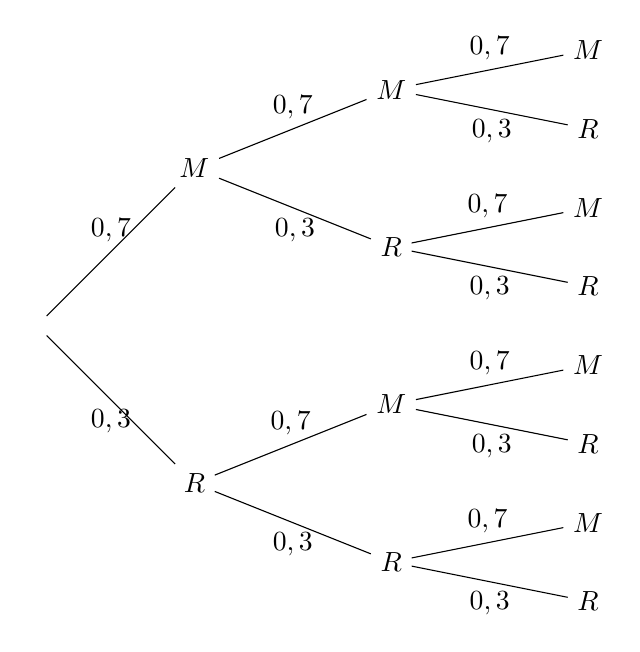
\begin{tikzpicture}
			[level 1/.style={level distance=2cm,
				sibling distance=4cm},
			level 2/.style={level distance=2.5cm,
				sibling distance=2cm},
			level 3/.style={level distance=2.5cm,
					sibling distance=1cm}]
			\node {} [grow'=right]
			child {node {$M$}
				child {node {$M$}
						child {node {$M$}
						edge from parent node[above] {$0,7$}
					}
					child {node {$R$}
						edge from parent node[below] {$0,3$}
					}
				edge from parent node[above] {$0,7$}
				}
				child {node {$R$}
						child {node {$M$}
						edge from parent node[above] {$0,7$}
					}
					child {node {$R$}
						edge from parent node[below] {$0,3$}
					}
				edge from parent node[below] {$0,3$}
				}
				edge from parent node[above] {$0,7$}
			}
			child {node {$R$}
				child {node {$M$}
						child {node {$M$}
						edge from parent node[above] {$0,7$}
					}
					child {node {$R$}
						edge from parent node[below] {$0,3$}
					}
					edge from parent node[above] {$0,7$}
				}
				child {node {$R$}
						child {node {$M$}
						edge from parent node[above] {$0,7$}
					}
					child {node {$R$}
						edge from parent node[below] {$0,3$}
					}
					edge from parent node[below] {$0,3$}
				}
				edge from parent node[below] {$0,3$}
			}
			;
		\end{tikzpicture}
	\end{center}

	
	\subsubsection*{b. Déterminer la loi de probabilité de $X$.}
	
	$X$ peut prendre les valeurs 0, 1, 2 et 3.
	
	\[
	\begin{array}{|c|c|c|c|c|}
		\hline
			X & 0 & 1 & 2 & 3 \\
		\hline
		P(X = x_i) & 0,027 & 0,189 & 0,441 & 0,343 \\
			\hline
	\end{array}
	\]
	
	\subsubsection*{c. Calculer l'espérance $\mathbb{E}(X)$ de la variable aléatoire $X$.}
	
	\[
	\mathbb{E}(X) = 0 \times 0,027 + 1 \times 0,189 + 2 \times 0,441 + 3 \times 0,343 = 0,189 + 0,882 + 1,029 = 2,100
	\]
	
	Sur un grand nombre de tirs, Karim en réussira 21 sur 30.
	
	\subsection*{2. On propose à un spectateur le jeu suivant : il mise 15 € avant la série de tirs au but de Karim ; chaque but marqué par Karim lui rapporte 6 €, et chaque but manqué par Karim ne lui rapporte rien.}
	
	\subsubsection*{a. Exprimer $Y$ en fonction de $X$.}
	
	On a $Y = 6X - 15$. Les valeurs de $Y$ sont donc : -15, -9, -3 et 3.
	
	\subsubsection*{b. Calculer l'espérance $\mathbb{E}(Y)$ de la variable aléatoire $Y$. Interpréter ce résultat dans le contexte de l'énoncé.}
	
	\[
	\mathbb{E}(Y) = -15 \times 0,027 - 9 \times 0,189 - 3 \times 0,441 + 3 \times 0,343 = -0,405 - 1,701 + 1,029 = -2,4
	\]
	
	Cela signifie qu'en moyenne sur un grand nombre de tirs, le spectateur perdra 2,40 € par série de trois tirs. Le jeu est inéquitable.
	
